% --
% Speech Commands dataset

\subsection{Speech Commands Dataset}
The Speech Command Dataset \cite{warden2018} is a very diverse dataset consisting of over thousands of different speakers. This dataset is by any means no clean dataset recorded by professionals, if anything it is the opposite. 
The audio files are not normalized, there are samples with inconsistent sample numbers and some examples are prone with too much noise or even noise only.
And its still great, because there is no need for a perfect dataset and one can be happy that there exists one with this amount of diversity and free of access.
In fact maybe its even better to have an unclean dataset, so that invariances against noise are learnt and do not have be added by hand.

\begin{figure}[!ht]
  \centering
    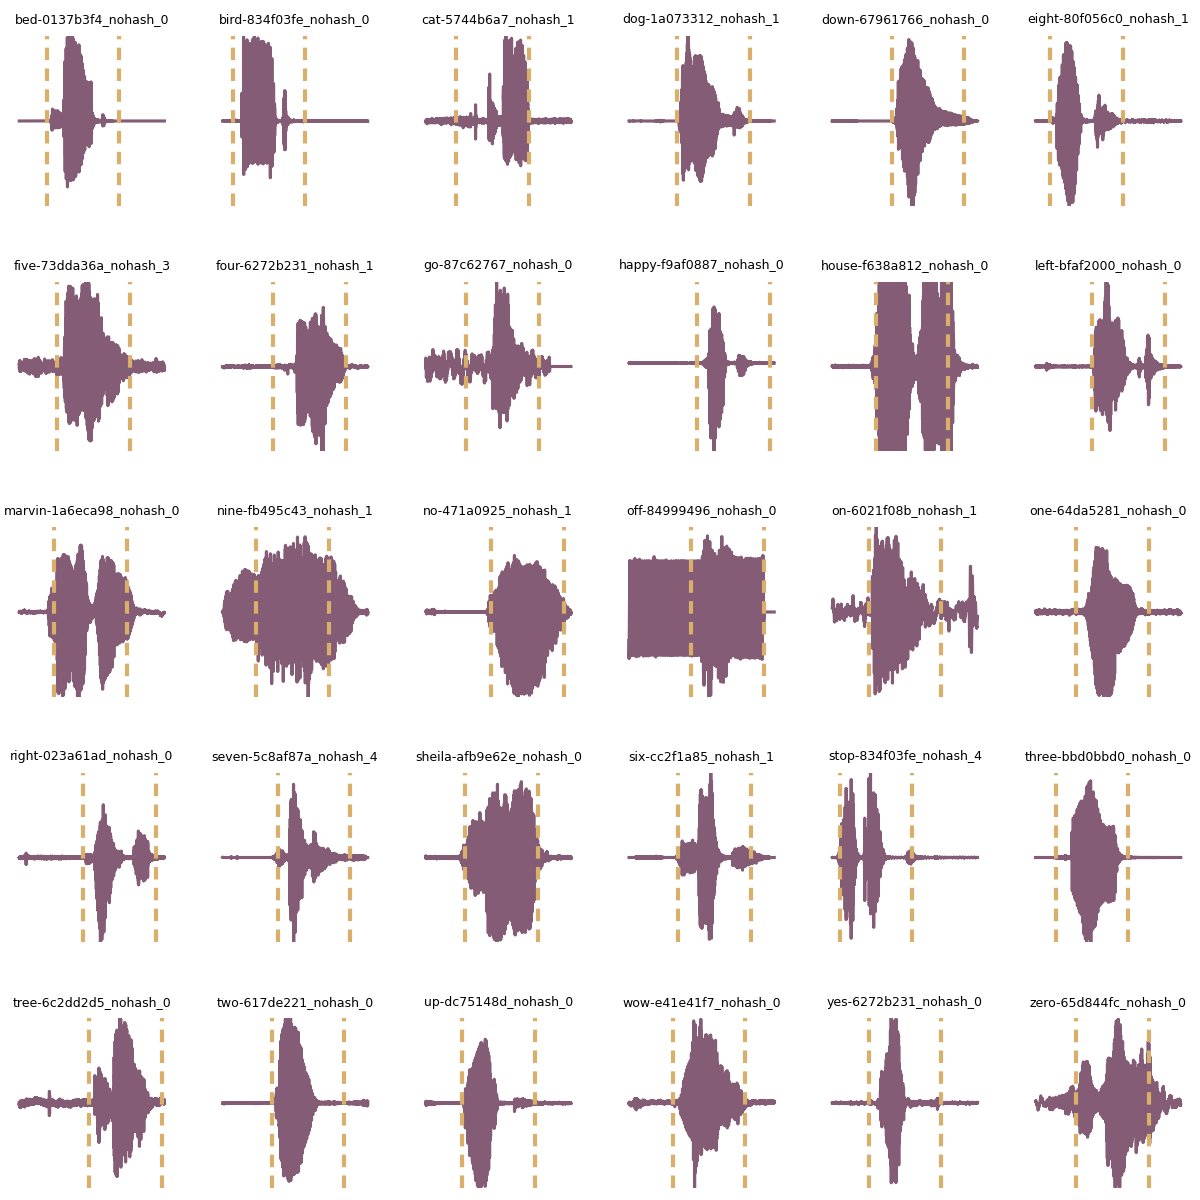
\includegraphics[width=0.65\textwidth]{./4_practice/figs/a_dataset/wav_grid_c30}
  \caption{Random samples from the Speech Command Dataset, one per class. Pre-processed and normalized raw audio data.}
  \label{fig:wav_grid_c30}
\end{figure}
\FloatBarrier
\noindent

\subsubsection{Extraction for Training}
The Speech Commands Dataset is extracted before it is used for training. 
To reduce computations in the evaluation process of Neural Networks, it was important to reduce the number of classes and examples per class to an suitable number.
In the Evaluation of Neural Networks the datasets the references in \rtab{dataset_refs} are used

\begin{table}[ht!]
\begin{center}
\caption{Dataset references with label restrictions in number of labels and labels itself.}
\begin{tabular}{ M{2cm}  M{2cm}  M{5cm} }
\toprule
%\multicolumn{4}{c}{\textbf{Feature Groups}} & \multicolumn{2}{c}{\textbf{Accuracy}} \\
\textbf{Reference name} & \textbf{Number of examples per label} & \textbf{Selected Labels}\\
\midrule
n500-c5 & 500 & left, right, up, down, go\\
n500-c10 & 500 & yes, no, left, go, down, off, right, stop, up, on\\
n500-c30 & 500 & \enquote{all}\\
\bottomrule
\label{tab:dataset_refs}
\end{tabular}
\end{center}
\end{table}
\FloatBarrier
\noindent
